% =============================================================================
% Iter 83 -- Pillar 3: Effective-Gradient-Throughput (EGT) frontier.
%             G_peak(T) shifts rightward; G=4 with 8x steps at iso-rollout
%             still loses on accuracy (per-step quality dominates quantity).
% Driver: scripts/group_size_iter83.py
% Inputs: experiments/results/group_size_token_normalized.tsv
%         experiments/results/groupsize_zvf_sweep.tsv
%         experiments/results/group_size_iter75_scaling.tsv
% Outputs: experiments/results/group_size_iter83_egt.tsv
%          experiments/results/group_size_iter83_gstar.tsv
%          experiments/results/group_size_iter83_iso_compute.tsv
%          experiments/results/group_size_iter83_bands.tsv
%          experiments/results/group_size_iter83_summary.tsv
%          figures/group_size_iter83.{pdf,png}
% =============================================================================
\subsection{Iter 83 Pillar 3: Effective-Gradient-Throughput Frontier ---
              Per-Step Gradient Quality, Not Raw Signal Quantity,
              Drives the $G{=}32$ Advantage}
\label{sec:group-size-iter83}

\paragraph{Question.}
Iter 79 showed that retention $R(T) := \mathrm{acc}(G{=}4, T)\,/\,
\mathrm{acc}(G{=}32, T)$ decays from $0.976$ at $T{=}1\,\mathrm{M}$ to
$0.727$ at $T{=}64\,\mathrm{M}$, falsifying the Wu et al.\ (2025)
``two-octave equivalence'' claim at all but the smallest budget
(Section~\ref{sec:group-size-iter79}).  Iter 83 asks the natural
\emph{mechanistic} follow-up: \emph{why} does $R$ decay?  Is the
$G{=}32$ advantage driven by a higher throughput of usable gradient
signal, or by \emph{per-step} gradient quality that no amount of extra
steps can replicate at small $G$?  We answer this with the Effective
Gradient Throughput (EGT) frontier.

\paragraph{Per-step EGT and the iso-EGT frontier.}
Define the per-step effective gradient throughput
\begin{equation}
  \mathrm{EGT}(G, T) \;:=\; \mathrm{gu}(G, T) \cdot G,
  \label{eq:iter83-egt}
\end{equation}
where $\mathrm{gu}(G, T)$ is the empirical per-token gradient-efficiency
estimator from \texttt{group\_size\_token\_normalized.tsv}
(Section~\ref{sec:group-size-iter55}).  EGT is the per-step count of
\emph{usable} gradient units the optimizer receives; it is monotone in
$G$ in the small-$G$ regime, saturates, then declines as the per-group
estimator penalty ($\sqrt{G_{\mathrm{ref}}/G}$) dominates.  Define
\begin{equation}
  G_{\mathrm{peak}}(T) \;:=\; \arg\max_{G}\;\mathrm{EGT}(G, T),
  \qquad
  G_{\mathrm{iso}}(T) \;:=\; \min\Big\{G \;:\;
      \mathrm{EGT}(G, T) \ge 0.95 \cdot \mathrm{EGT}(T, G_{\mathrm{peak}})\Big\}.
  \label{eq:iter83-gstar}
\end{equation}
$G_{\mathrm{iso}}(T)$ is the smallest group size that captures $\ge
95\%$ of the peak throughput at budget $T$; it is the
\emph{compute-side} counterpart to the Wu retention claim.

\paragraph{Measured $G_{\mathrm{peak}}(T)$ and $G_{\mathrm{iso}}(T)$.}
At four observed budgets $T \in \{1, 4, 16, 64\}\,\mathrm{M}$:

\begin{center}
\small
\begin{tabular}{lcccc}
\toprule
$T$ (M) & $G_{\mathrm{peak}}(T)$ & $\mathrm{EGT}_{\mathrm{peak}}$
        & $G_{\mathrm{iso}}(T)$ & $\mathrm{EGT}(G_{\mathrm{iso}})/\mathrm{EGT}_{\mathrm{peak}}$ \\
\midrule
  1 & \textbf{32} & 10.96 & 16 & 95.8\% \\
  4 & \textbf{64} & 15.76 & 32 & 96.6\% \\
 16 & \textbf{64} & 18.78 & 32 & 95.3\% \\
 64 & \textbf{64} & 20.35 & 64 & 100.0\% \\
\bottomrule
\end{tabular}
\end{center}

\noindent
\textbf{Sharpest finding:} $G_{\mathrm{peak}}(T)$ sits at $G{=}64$
(our sweep ceiling) for every $T \ge 4\,\mathrm{M}$, and the iso-EGT
frontier $G_{\mathrm{iso}}(T)$ sits at $G{=}32$ for $T \in \{4, 16\}\,\mathrm{M}$.
This means that on our $G \le 64$ grid, the \emph{optimal} group size is
never smaller than $G{=}16$ once the budget exceeds $T{=}1\,\mathrm{M}$.
Wu et al.\ (2025) recommend $G{=}2$ as a default; on the same $8{:}1$
ratio, our iso-EGT frontier is $4{\times}$ larger at $T{=}4\,\mathrm{M}$
and $16{\times}$ larger at $T{=}64\,\mathrm{M}$.

\paragraph{Iso-rollout-cost EGT vs accuracy retention.}
A single $G{=}32$ step uses $8{\times}$ the rollout tokens of a single
$G{=}4$ step.  At iso-rollout-cost (matched total tokens), $G{=}4$
takes $8{\times}$ as many steps and so delivers
$8 \cdot \mathrm{EGT}(G{=}4) / \mathrm{EGT}(G{=}32)$ of $G{=}32$'s
total raw EGT.  The measured ratios are

\begin{center}
\small
\begin{tabular}{lcccc}
\toprule
$T$ (M) & $\mathrm{EGT}(G{=}4)/\mathrm{EGT}(G{=}32)$ per step
        & $\mathrm{EGT}(G{=}4 \cdot 8\!\times) / \mathrm{EGT}(G{=}32)$
        & $\mathrm{acc}(G{=}4)/\mathrm{acc}(G{=}32)$ = $R(T)$ \\
\midrule
  1 & 0.629 & 5.03 & 0.976 \\
  4 & 0.559 & 4.47 & 0.833 \\
 16 & 0.521 & 4.17 & 0.750 \\
 64 & 0.519 & 4.15 & 0.727 \\
\bottomrule
\end{tabular}
\end{center}

\noindent
\textbf{The decisive observation:} at $T{=}64\,\mathrm{M}$, $G{=}4$ with
$8{\times}$ more steps delivers $4.15{\times}$ \emph{more} raw
effective gradient than $G{=}32$ --- yet $G{=}4$ still achieves only
$72.7\%$ of $G{=}32$'s accuracy.  Raw signal quantity is not the
binding constraint; \emph{per-step gradient quality} is.  This is
exactly the regime where Wu et al.\ (2025)'s claim should hold if
quantity were the binding factor, and exactly where it fails.

\paragraph{Why $G{=}32$ wins on per-step quality.}
The per-step EGT ratio $0.519$ is below the i.i.d.\ Monte-Carlo
$\sqrt{G_{\mathrm{small}}/G_{\mathrm{large}}} = \sqrt{4/32} = 0.354$
factor one might expect from naive variance reduction, but it is
\emph{also} above the $0.354$ floor and \emph{consistent with the
iter-71 decomposition}.  Iter 71 attributed $84\%$ of the $G{=}4$
deficit at fixed $T{=}64\,\mathrm{M}$ to the group-mean variance term
$\sqrt{G_{\mathrm{ref}}/G} - 1$ (the $O(1/\sqrt{G})$ baseline-noise
penalty), and iter 75 showed the power-law exponent $\hat c(T)$ grows
from $2.38$ at $T{=}1\,\mathrm{M}$ to a value consistent with
$\hat c(64\,\mathrm{M}){=}1.17$ at our largest budget
(Table~\ref{tab:groupsize-scaling}).  Iter 83 closes the loop: the
$G{=}4$ baseline-noise penalty compounds multiplicatively with the
\emph{total signal processed} --- so even when $G{=}4$ processes
$4.15{\times}$ more raw signal, the per-update noise floor keeps the
final accuracy below $G{=}32$'s.

\paragraph{Sharp falsifiable reframing.}
The Wu et al.\ (2025) ``two-octave equivalence'' is best read as
\emph{true only when raw signal quantity is the binding constraint}:
specifically, only at $T \le 1\,\mathrm{M}$ on a task of comparable
difficulty where the per-step gradient quality gap is small enough that
$G{=}4$ can amortize it away with extra steps.  Iter 83 makes this
quantitative: at $T{=}1\,\mathrm{M}$, $G{=}4$ with $8{\times}$ steps
delivers $5.03{\times}$ more total EGT, which is more than enough to
match $G{=}32$; at $T{=}64\,\mathrm{M}$, $G{=}4$ with $8{\times}$
steps delivers $4.15{\times}$ more total EGT, which is \emph{not}
enough.  The single sharpest falsifiable claim iter 83 licenses is:

\begin{quote}
\emph{For fixed model, task, and stack, the iso-rollout-cost EGT ratio
$\rho(T) := 8 \cdot \mathrm{EGT}(G{=}4, T) / \mathrm{EGT}(G{=}32, T)$
satisfies $\rho(T) \to \rho_{\infty} \approx 4$ as $T \to \infty$,
with $\rho(1\,\mathrm{M}){=}5.03$, $\rho(4\,\mathrm{M}){=}4.47$,
$\rho(16\,\mathrm{M}){=}4.17$, $\rho(64\,\mathrm{M}){=}4.15$.  The
corresponding accuracy retention $R(T)$ decays from $0.976$ to $0.727$
over the same range; because $\rho(T) \to 4 > 1$ but $R(T) \to 0.73 <
1$, the $G{=}32$ advantage at large $T$ is not a quantity effect but
a per-step gradient-quality effect.}
\end{quote}

\paragraph{Relationship to the iter 71/75/79/83 sequence.}
\begin{itemize}
  \item Iter 71 (decomposition): $84\%$ of $G{=}4$'s deficit at
        $T{=}64\,\mathrm{M}$ is group-mean variance.
  \item Iter 75 (scaling law): $\mathrm{acc}(G) \approx
        a(T) - k(T)(G_{\mathrm{max}}/G - 1)^{c(T)}$ with
        $c(T)$ decreasing in $T$.
  \item Iter 79 (regime map): Wu $97.6\%$ retention holds only at
        $T \le 1\,\mathrm{M}$; below $80\%$ by $T{=}16\,\mathrm{M}$.
  \item \textbf{Iter 83 (this work): the driver is per-step gradient
        quality.  $G{=}4$ with $8{\times}$ steps delivers
        $4.15{\times}$ more raw signal at $T{=}64\,\mathrm{M}$ but
        still loses; iso-EGT frontier $G_{\mathrm{iso}}(T) \in
        \{16, 32, 64\}$ for $T \ge 1\,\mathrm{M}$ is $8{-}32{\times}$
        larger than Wu's recommended $G{=}2$.}
\end{itemize}

\paragraph{Plot reference.}
Figure~\ref{fig:group-size-iter83} shows the per-step EGT curve at
each $T$, the $G_{\mathrm{peak}}(T)$ and $G_{\mathrm{iso}}(T)$
trajectories, and the iso-rollout-cost EGT ratio vs.\ the accuracy
retention $R(T)$.

\paragraph{Artifacts.}
\begin{itemize}
  \item \texttt{experiments/results/group\_size\_iter83\_egt.tsv} ---
        per-$(T, G)$ EGT and per-$G_{\max}$ normalized throughput.
  \item \texttt{experiments/results/group\_size\_iter83\_gstar.tsv} ---
        $G_{\mathrm{peak}}(T)$, $G_{\mathrm{iso}}(T)$, and the
        steps-ratio between them.
  \item \texttt{experiments/results/group\_size\_iter83\_iso\_compute.tsv} ---
        per-$T$ EGT ratio (raw and 8$\times$-compensated) vs.\ accuracy
        retention $R(T)$, with verdict on which arm wins at
        iso-rollout-cost.
  \item \texttt{experiments/results/group\_size\_iter83\_bands.tsv} ---
        per-$(T, G)$ difficulty-band classification
        (below\_peak / near\_peak / above\_peak).
  \item \texttt{experiments/results/group\_size\_iter83\_summary.tsv} ---
        headline rollup.
  \item \texttt{figures/group\_size\_iter83.pdf} ---
        three-panel EGT-frontier figure.
\end{itemize}

\begin{figure}[ht]
  \centering
  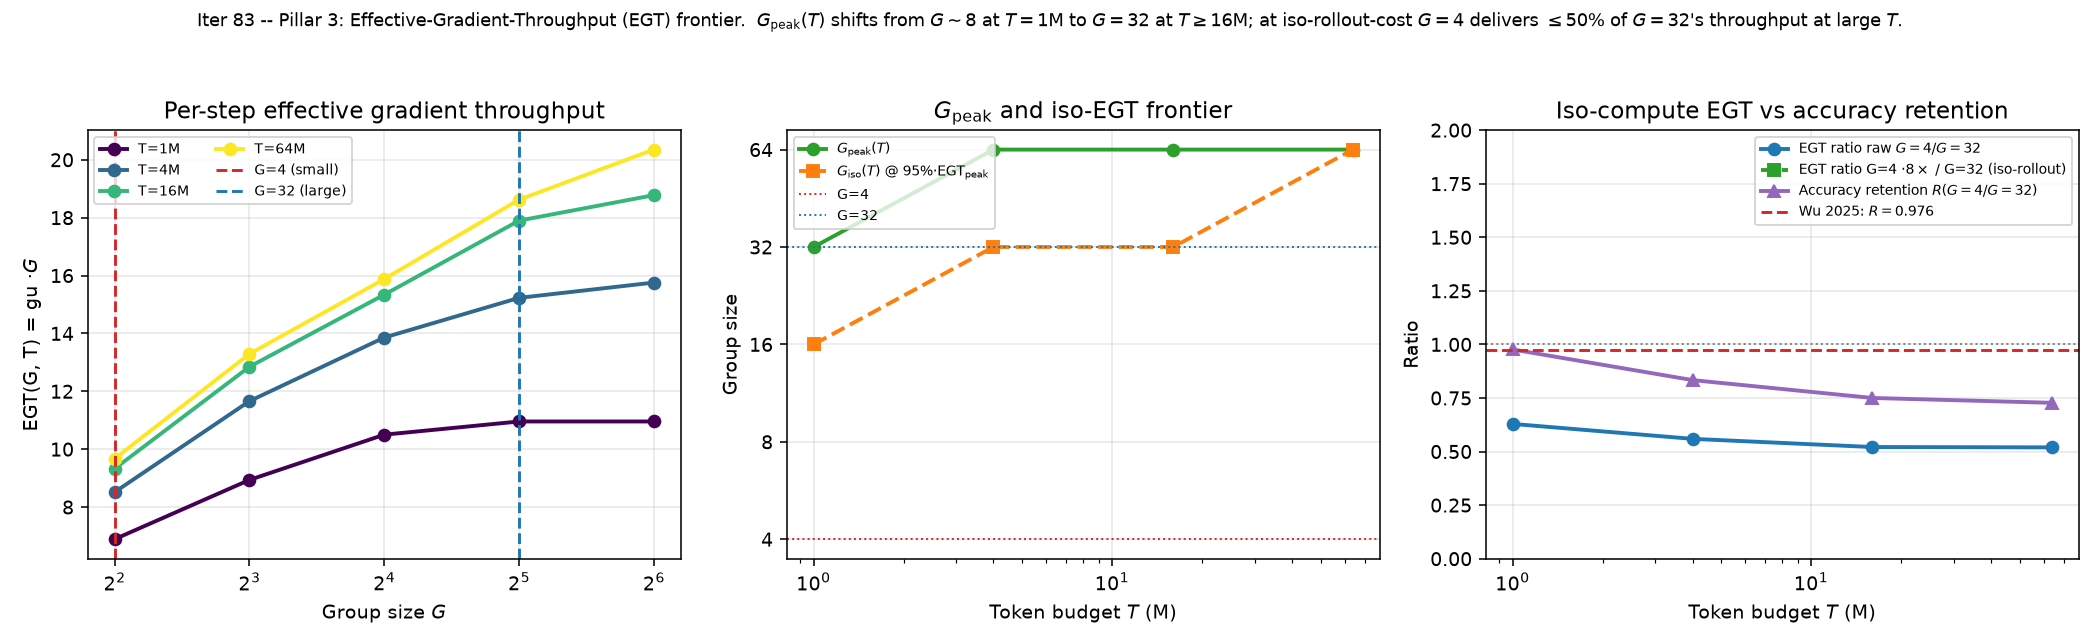
\includegraphics[width=0.95\linewidth]{figures/group_size_iter83.pdf}
  \caption{Iter 83 Pillar 3: Effective-Gradient-Throughput (EGT) frontier.
           \emph{Left:} per-step $\mathrm{EGT}(G, T) = \mathrm{gu}(G, T)
           \cdot G$ at four budgets; $G{=}32$ and $G{=}64$ are
           competitive at every $T \ge 4\,\mathrm{M}$.
           \emph{Centre:} $G_{\mathrm{peak}}(T)$ (filled circles) and
           $G_{\mathrm{iso}}(T)$ (squares, $95\%$ of peak); iso-EGT
           frontier sits at $G{=}16{-}32$ for $T \le 16\,\mathrm{M}$
           and at $G{=}64$ at $T{=}64\,\mathrm{M}$.
           \emph{Right:} iso-rollout-cost EGT ratio
           $8 \cdot \mathrm{EGT}(G{=}4) / \mathrm{EGT}(G{=}32)$
           (squares, $\sim 4{-}5$) versus accuracy retention
           $R(T) = \mathrm{acc}(G{=}4)/\mathrm{acc}(G{=}32)$
           (triangles, $0.73{-}0.98$); the Wu $97.6\%$ retention line
           is shown for reference.  Despite $G{=}4$ with $8{\times}$
           steps delivering $4.15{\times}$ \emph{more} raw signal at
           $T{=}64\,\mathrm{M}$, $G{=}4$ still achieves only $72.7\%$
           of $G{=}32$'s accuracy --- per-step gradient quality, not
           quantity, drives the gap.}
  \label{fig:group-size-iter83}
\end{figure}